\documentclass[a4paper,14pt]{extarticle}
\usepackage[utf8]{inputenc}
\usepackage[russian]{babel}
\usepackage{graphicx}
\usepackage[top=0.8in, bottom=0.8in, left=0.8in, right=0.8in]
{geometry}
\usepackage{pgfplots}
\usepackage{amsmath}
\usepackage{setspace}
\usepackage{titlesec}
\usepackage{float}
\usepackage{chngcntr}
\usepackage{pgfplots}
\usepackage{amsfonts}
\usepackage{pgfplotstable}
\usepackage{multirow}
\usepackage{karnaugh-map}
\usepackage{tikz,xcolor}
\usepackage{indentfirst} % Красная строка
\usepackage{listings}
\usepackage{amssymb}
\usepackage{xcolor}
\usepackage{hyperref}

\titleformat{\section}[hang]
  {\bfseries}
  {}
  {0em}
  {\hspace{-0.4pt}\large \thesection\hspace{0.6em}}
  
  
\titleformat{\subsection}[hang]
  {\bfseries}
  {}
  {0em}
  {\hspace{-0.4pt}\large \thesubsection\hspace{0.6em}}

%\linespread{1.3} % полуторный интервал
%\renewcommand{\rmdefault}{ftm} % Times New Roman

\newcommand{\nx}{\overline{x}}
\newcommand{\p}{0.31}
\newcommand{\scale}{1.4}

\counterwithin{figure}{section}
\counterwithin{equation}{section}
\counterwithin{table}{section}

\begin{document}
\begin{titlepage}
\centering
Санкт-Петербургский политехнический университет Петра Великого \\
\vspace{0.15cm}
Кафедра компьютерных систем и программных технологий \\
\vspace{6.5cm}

{\centering \textbf{Отчёт по лабораторной работе} \\ 
\vspace{0.15cm}
\textbf{Дисциплина}: Телекоммуникационные технологии \\
\vspace{0.15cm}
\textbf{Тема}: Сигналы телекоммуникационных. Преобразование Фурье. Корреляция
систем} \\

\vspace{6.5cm}

\begin{table}[H]
\begin{tabular}{p{\textwidth}@{}r}
{Выполнил студент гр. 33501/2} \hfill {Вахаев И.Н.} \\
{Преподаватель} \hfill {Богач Н.В.} \\
\end{tabular}
\end{table}
\vfill

{\centering Санкт-Петербург \\ 
\vspace{0.15cm}
\today}
\end{titlepage}

\tableofcontents
\newpage

\section{Цель работы}

Познакомиться со средствами генерации и визуализации простых сигналов.
Получить представление о спектрах теллекомуникационных сигналов.

\section{Постановка задачи}


\begin{itemize}
\item В командном окне MATLAB и в среде Simulink промоделировать синусоидальный и прямоугольный сигналы с различными параметрами. Получить их спектры. Вывести на график.
\item Для сигналов, построенных в лабораторной работе №1, выполните расчет преобразования Фурье. Перечислите свойства преобразования Фурье.
\item С помощью функции корреляции найдите позицию синхропосылки [101] в сигнале [0001010111000010]. Получите пакет
данных, если известно, что его длина составляет 8 бит без учета синхропосылки. Вычислите корреляцию прямым методом, воспользуйтесь алгоритмом быстрой корреляции, сравните время работы обоих алгоритмов.
\item Быстрая корреляция
\end{itemize}

\section{Теория}

\subsection{Сигналы}

\textbf{Простой сигнал} -- это одиночный импульс или последовательность импульсов.\\

Все одиночные радиоимпульсы с произвольной формой огибающей, их последовательности, т.е. «пачки» радиоимпульсов, не имеющих глубокой фазовой или частотной модуляции (манипуляции), относятся к классу простых сигналов.

\textbf{Классификация сигналов:}
\begin{enumerate}
\item По физической природе носителя информации:
	\begin{itemize}
	\item электрические
	\item электромагнитные
	\item оптические
	\item акустические
	\item и другие
	\end{itemize}
\item По способу задания сигнала:
	\begin{itemize}
	\item регулярный/детерминированные, заданные аналитической функцией
	\item нерегулярные/случайные, принимающие произвольные значения в любой момент времени. Для описания таких сигналов используется аппарат теории вероятностей.
	\end{itemize}
\item В зависимости от функции, описывающей параметры сигнала, выделяют аналоговые, дискретные, квантованные и цифровые сигналы:
	\begin{itemize}
\item непрерывные (аналоговые), описываемые непрерывной функцией
\item дискретные, описываемые функцией отсчётов, взятых в определённые моменты времени;
\item квантованные по уровню;
\item дискретные сигналы, квантованные по уровню (цифровые).
	\end{itemize}
	\end{enumerate}

\subsection{Преобразования Фурье}

Преобразования Фурье осуществляется с помощью ряда Фурье и с 
помощью интеграла Фурье, причём первый применяется когда функция 
периодическая, а второй когда она апериодична.\\

Любая ограниченная, периодическая функция, имеющая конечное число экстремумов на протяжении периода, может быть представлена в виде ряда Фурье:
\begin{equation}
\varphi_{p}(t) = \sum\limits_{k=-\infty}^\infty C_{k}e^{j2 \pi kf_{1}t}
\end{equation}

где $f_{1} = 1/T_{1}; T_{1}$ - период функции $\varphi_{p}(t)$; $C_{k}$ - постоянные коэффициенты.\\
Коэффициенты находятся по следующей формуле:

\begin{equation}
C_{k} = \dfrac{1}{T_{1}} \int_{t_{0}}^{t_{0}+T_{1}} \varphi_{p}(t)e^{-j \pi kf_{1}t} dt
\end{equation}
Значение выражения не зависит от $t_{0}$. Как правило, берется $t_{0}=0$ или $t_{0}= -T_{1}/2$.

Приведенные формулы можно записать в виде одного выражения:
\begin{equation}
\varphi_{p}(t) = \sum\limits_{k=-\infty}^\infty \left[\frac{1}{T_{1}} \int_{t_{0}}^{t_{0}+T_{1}} \varphi_{p}(t)e^{-j \pi kf_{1}t} dt\right] e^{j2 \pi kf_{1}t}
\end{equation}

Ряд Фурье справедлив для периодических сигналов, однако на его основе можно вывести соотношения и для непериодических сигналов. В этом случае период $T_{1}\rightarrow \infty$, в связи с этим частота $f_{1}\rightarrow0$ и обозначается как $df, kf_{1}$ является текущим значением частоты f, а сумма меняется на интеграл. В результате получается выражение:
\begin{equation}
\varphi_{p}(t)= \int_{-\infty}^{\infty} \left[ \int_{-\infty}^{\infty} \varphi_{p}(t)e^{-j2 \pi ft} dt\right] e^{j2 \pi ft} df.
\end{equation}
Это выражение называется интегралом Фурье и объединяет прямое преобразование Фурье:

\begin{equation}
\Phi(f) = \int_{-\infty}^{\infty} \varphi_{p}(t)e^{-j2 \pi ft} dt
\end{equation}

с обратным преобразованием Фурье:
\begin{equation}
\varphi(t) = \int_{-\infty}^{\infty} \Phi(f) e^{j2 \pi ft} dt.
\end{equation}

Приведенные преобразования существуют только для функций с ограниченной энергией:
\begin{equation}
\int_{-\infty}^{\infty} \rvert \varphi(t) \rvert^{2} dt \neq \infty
\end{equation}

В большинстве случаев термин преобразование Фурье обозначает именно интеграл Фурье. Преобразование Фурье сигнала ещё называют спектром сигнала.

\subsection{Свойства преобразования Фурье}

Преобразование Фурье имеет следующие свойства:

\begin{itemize}
	\item Смещение функций.
\end{itemize}
При смещении функции на $t_{0}$ ее Преобразование Фурье умножается на $e^{j2 \pi f t_{0}}$

\begin{itemize}
	\item Суммирование функций.
\end{itemize}
Преобразование Фурье – линейное преобразование. Отсюда следует:
\begin{equation}
\sum\limits_{i=1}^{n} \alpha_{i} \varphi_{i} (t) \leftrightarrow \sum\limits_{i=1}^{n} \alpha_{i} \Phi_{i} (f)
\end{equation}
где $\alpha_{i}$ постоянный коэффициент.

\begin{equation}
\varphi(t-t_{0}) \leftrightarrow e^{-j2 \pi f t_{0}}\Phi(f).
\end{equation}

\begin{itemize}
	\item Свертывание функций.
\end{itemize}
Преобразование Фурье свертки двух функций равно произведению Преобразований Фурье этих функций:

\begin{itemize}
	\item Перемножение функций.
\end{itemize}
Преобразование Фурье произведения двух функции равно свертке Преобразований Фурье этих функций:

\begin{equation}
\varphi_{1} (t) \varphi_{2} (t) \leftrightarrow \Phi_{1} (f) * \Phi_{2} (f).
\end{equation}

\begin{itemize}
	\item Изменение масштаба аргумента функции.
\end{itemize}
При домножении аргумента функции $t$ на постоянный коэффициент $\alpha$, Преобразование Фурье функции имеет вид $\frac{1}{\mid\alpha\mid} \Phi (\frac{f}{\alpha}):$

\begin{equation}
\varphi(\alpha t) \leftrightarrow \frac{1}{\alpha} \Phi \left(\frac{f}{\alpha} \right)
\end{equation}

\begin{equation}
\varphi_{1} (t) * \varphi_{2} (t) \leftrightarrow \Phi_{1} (f) \Phi_{2} (f).
\end{equation}

\begin{itemize}
	\item Обратимость преобразования.
\end{itemize}
Преобразование обратимо с точность до знака аргумента.

\begin{equation}
\varphi (t) \leftarrow \Phi (f)
\end{equation}
\begin{equation}
\Phi(t) \leftrightarrow \varphi(-f), \Phi (-t) \leftrightarrow \varphi (f)
\end{equation}

\begin{itemize}
	\item Дифференцирование функции.
\end{itemize}
При дифференцировании функции ее ПФ домножается на $j2 \pi f $:

\begin{equation}
\dfrac{d[\varphi (t)]}{dt}\leftrightarrow j2 \pi f \Phi (f)
\end{equation}

\begin{itemize}
	\item Интегрирование функции.
\end{itemize}
При интегрировании функции ее Преобразование Фурье делится на $j2 \pi f :$

\begin{equation}
\int_{-\infty}^{t} \varphi(t') dt' \leftrightarrow \dfrac{1}{j2 \pi f} \Phi (f)
\end{equation}


\subsection{Корреляция сигналов}

Корреляция является методом анализа сигналов.

Корреляционный анализ дает возможность установить в сигналах (или в рядах цифровых данных сигналов) наличие определенной связи изменения значений сигналов по независимой переменной, когда большие значения одного сигнала связаны с большими значениями другого сигнала (положительная корреляция), или малые значения одного сигнала связаны с большими значениями другого (отрицательная корреляция), или данные двух сигналов никак не связаны (нулевая корреляция).

Чтобы найти посылку в сигнале зачастую используется алгоритм взаимной корреляции, где N- длинна всех х и у. Для этого сдвигается один вектор относительно другого, при этом каждый раз находя значение корреляции. Там, где значение корреляции будет максимальным, будет находиться искомая посылка:

\begin{equation}
R = \frac{1}{N} \sum\limits_{i=1}^{N} x_{i}* y_{i} 
\end{equation}

Алгоритм быстрой корреляции выглядит следующим образом:

\begin{equation}
R = \frac{1}{N} F_{d}^{-1} [X's * Y] 
\end{equation}


\section{Ход работы}

\subsection{Моделирование синусоидального сигнала}

\subsubsection{Получение непрерывного сигнала}

После открытия Matlab запускаем Simulink, иконку которого можно увидеть на верхней панели стартового окна

\begin{figure}[H]
\center{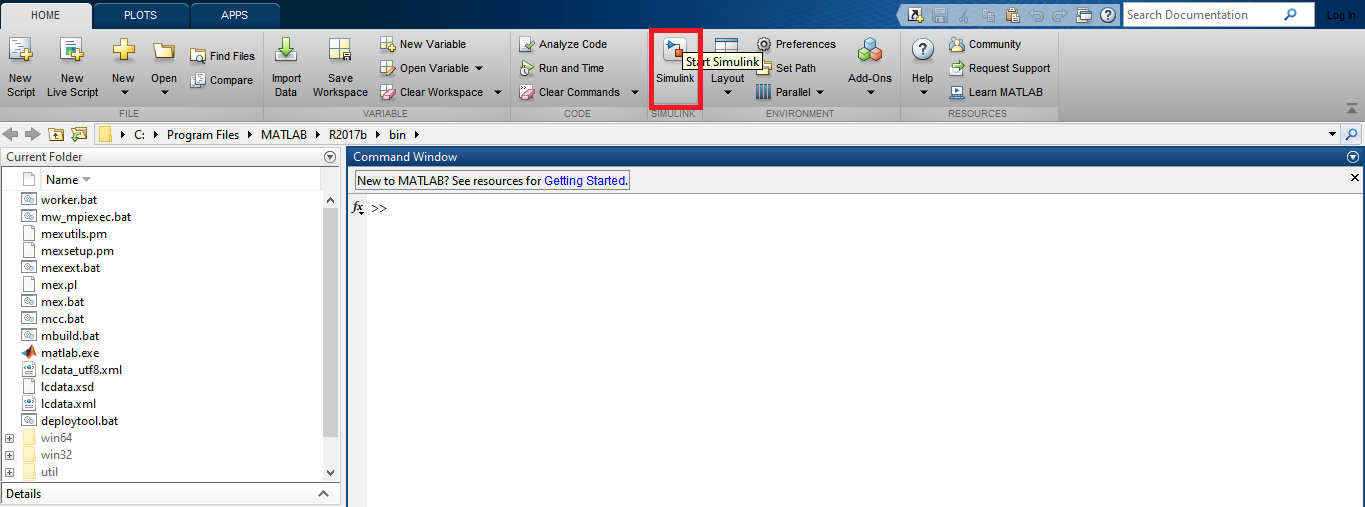
\includegraphics[width=0.5\linewidth]{screen/000.png}}
\caption{Выбор ячейки Simulink.}
\end{figure}

Был выбран шаблон Blank Model для начала необходимой работы в Simulink 

\begin{figure}[H]
\center{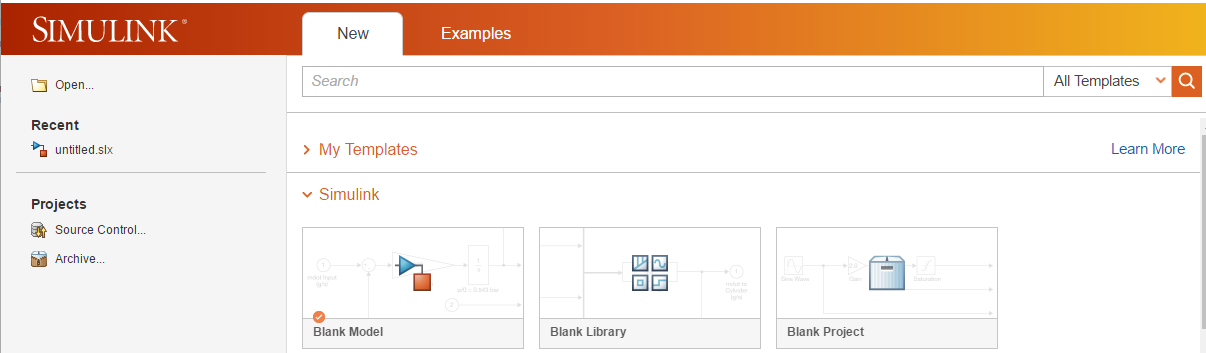
\includegraphics[width=0.5\linewidth]{screen/001.png}}
\caption{Выбор шаблона в начальном окне Simulink.}
\label{001}
\end{figure}

Затем была открыта вкладка Library Browser, в которой мы нашли следующие элементы: Sine Wave, Scope.

\begin{figure}[H]
\center{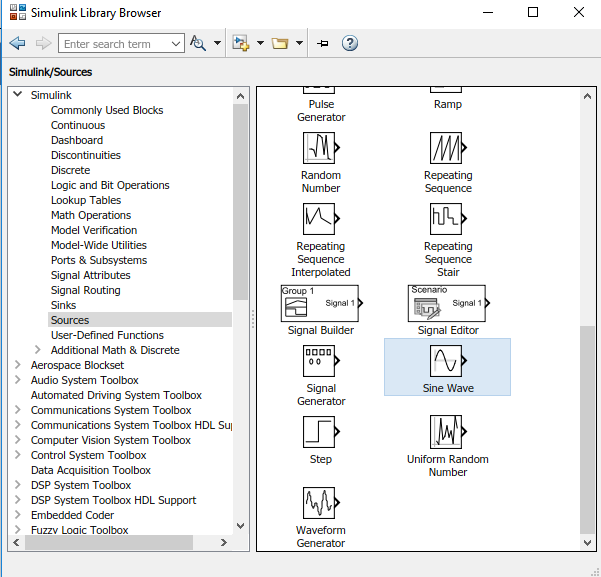
\includegraphics[width=0.5\linewidth]{screen/002.png}}
\caption{Поиск необходимых элементов в библиотеке.}
\label{002}
\end{figure}

Получили следующую схему:

\begin{figure}[H]
\center{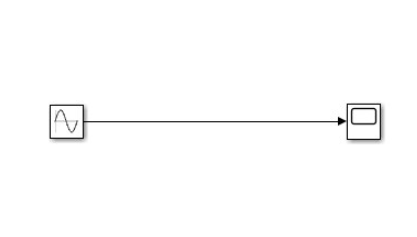
\includegraphics[width=0.5\linewidth]{screen/008.png}}
\caption{Схема, необходимая для симуляции синусоидального сигнала.}
\label{008}
\end{figure}

В дальнейшем нам понадобится добавить ещё один элемент - Spectrum Analyzer.

Назначение элементов:
\begin{itemize}
\item \textbf{Sine Wave} для задания синусоидального сигнал с амплитудой 1 и частотой 1 rad/sec
\item \textbf{Scope} для принятия и визуализации полученного сигнала
\item \textbf{Spectrum Analyzer} для получения спектра сигнала\\
\end{itemize}

После запуска симуляции получим синусоидальный сигнал в окне Scope:

\begin{figure}[H]
\center{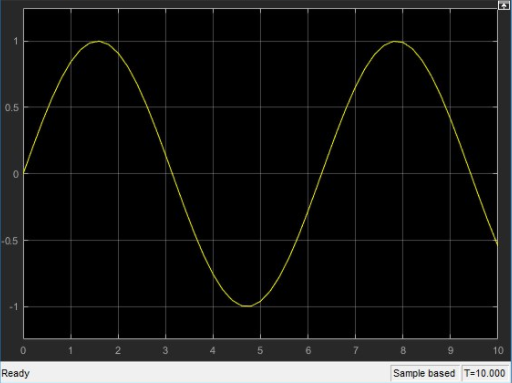
\includegraphics[width=0.5\linewidth]{screen/007.png}}
\caption{Синусоидальный сигнал.}
\label{007}
\end{figure}

\subsubsection{Получение дискретного сигнала}

Чтобы получить из непрерывного сигнала дискретный, нам необходимо изменить для элемента \textbf{Sine Wave} параметр $Sine \ type$ с $Time \ based$ на $Sample \ based$. Установим $Samples \ per \ period$ на $250\pi$, а $\ Sample \ time$ на $0.01$.

\begin{figure}[H]
\center{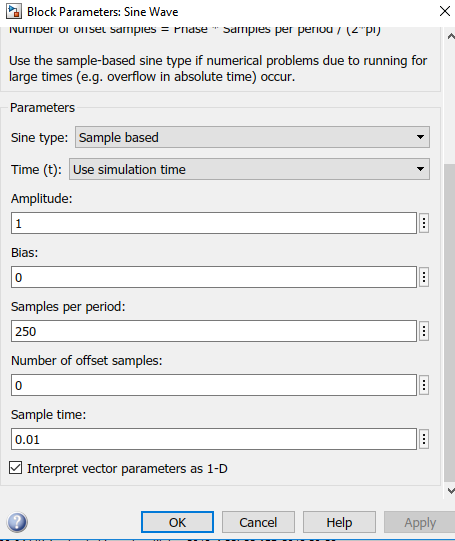
\includegraphics[width=0.5\linewidth]{screen/009a.png}}
\caption{Параметры синусоидального сигнала.}
\label{009a}
\end{figure}

После запуска симуляции мы получим необходимый нам синусоидальный дискретный сигнал

\begin{figure}[H]
\center{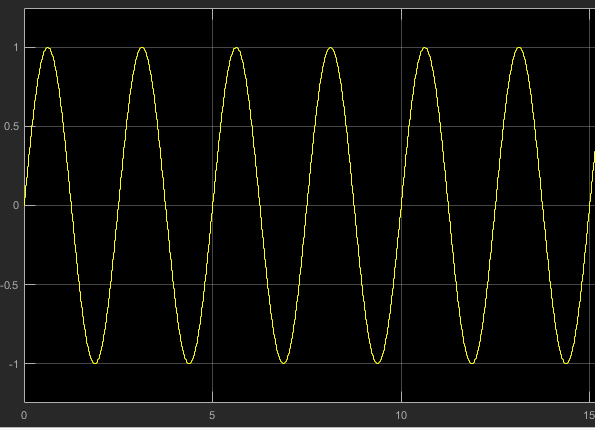
\includegraphics[width=0.5\linewidth]{screen/010.png}}
\caption{Дискретный синусоидальный сигнал.}
\label{010}
\end{figure}

\subsubsection{Получение спектра дискретного сигнала}

Для получения спектра дискретного сигнала добавим на схему элемент Spectrum Analyzer.

\begin{figure}[H]
\center{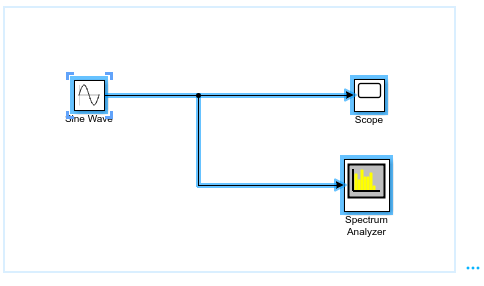
\includegraphics[width=0.5\linewidth]{screen/003.png}}
\caption{Схема для получения спектра.}
\label{003}
\end{figure}

Также для получения спектра дискретного сигнала установим $Sample \ time$ на 0.01 и $Simulation \ stop \ time$ на 20.

Запустив симуляцию, получим следующий результат:

\begin{figure}[H]
\center{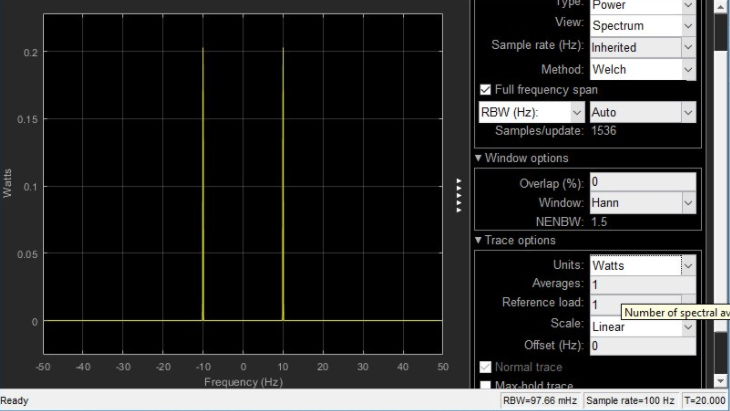
\includegraphics[width=0.5\linewidth]{screen/006.png}}
\caption{Спектрального представление синусоидального дискретного сигнала.}
\label{006}
\end{figure}

Изменим амплитуду входного сигнала с 1 до 10. Снова промодулируем сигнал.

\begin{figure}[H]
\center{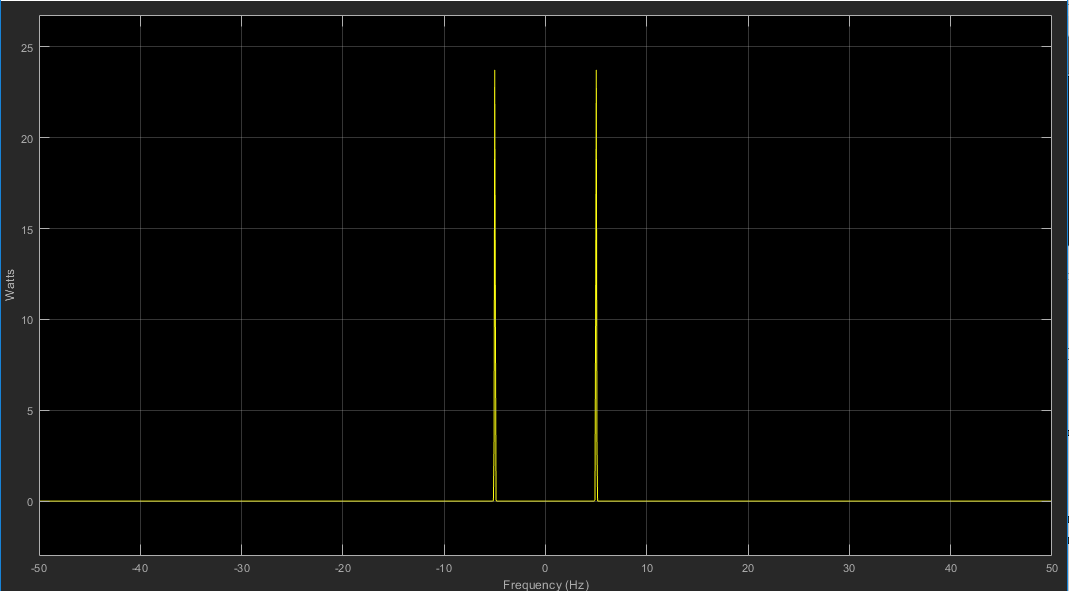
\includegraphics[width=0.5\linewidth]{screen/011.png}}
\caption{Спектрального представление синусоидального дискретного сигнала.}
\label{011}
\end{figure}

Изменим $Samples \ per \ period$ на значение $50\pi$

\begin{figure}[H]
\center{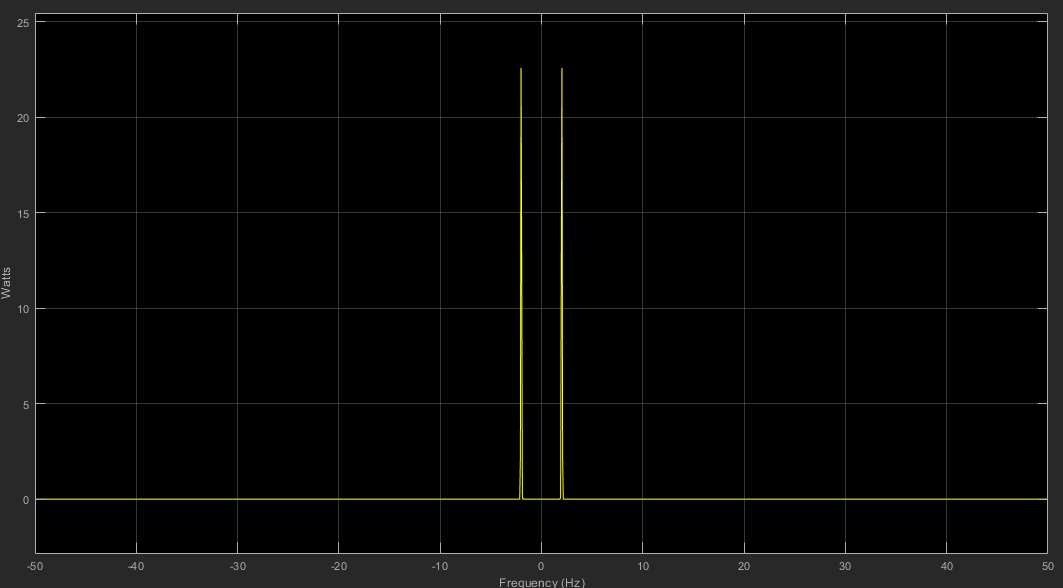
\includegraphics[width=0.5\linewidth]{screen/012.png}}
\caption{Спектрального представление синусоидального дискретного сигнала.}
\label{012}
\end{figure}

На рисунках \ref{006}, \ref{011}, \ref{012} показано, что при изменение периода обратно пропорционально изменяется частота спектра, а при изменение амплитуды сигнала линейно изменяется амплитуда спектра.

\subsection{Моделирование прямоугольного сигнала}

\subsubsection{Получение дискретного сигнала}

На рисунке \ref{013} представлена схема для исследования прямоугольного дискретного сигнала.

\begin{figure}[H]
\center{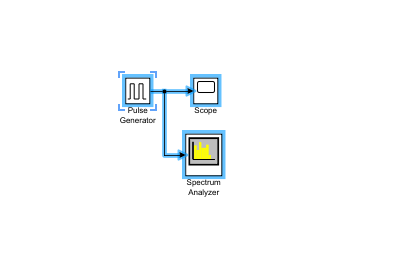
\includegraphics[width=0.5\linewidth]{screen/013.png}}
\caption{Схема для исследования прямоугольного дискретного сигнала.}
\label{013}
\end{figure}

На рисунке \ref{009} заданы параметры для \textbf{Pulse Generator}.

\begin{figure}[H]
\center{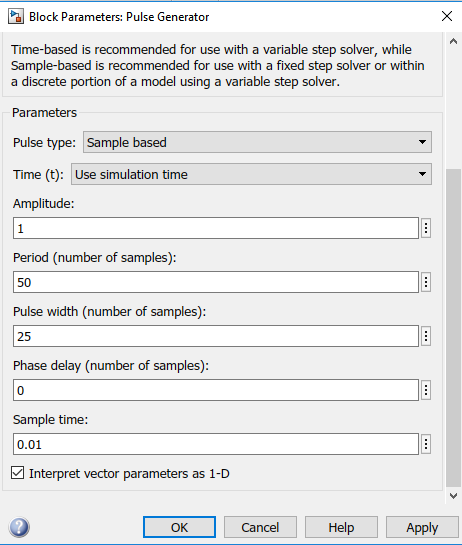
\includegraphics[width=0.5\linewidth]{screen/014.png}}
\caption{Схема для исследования прямоугольного дискретного сигнала.}
\label{014}
\end{figure}

После моделирования на рисунке \ref{010} были получены результаты(окно Scope).

\begin{figure}[H]
\center{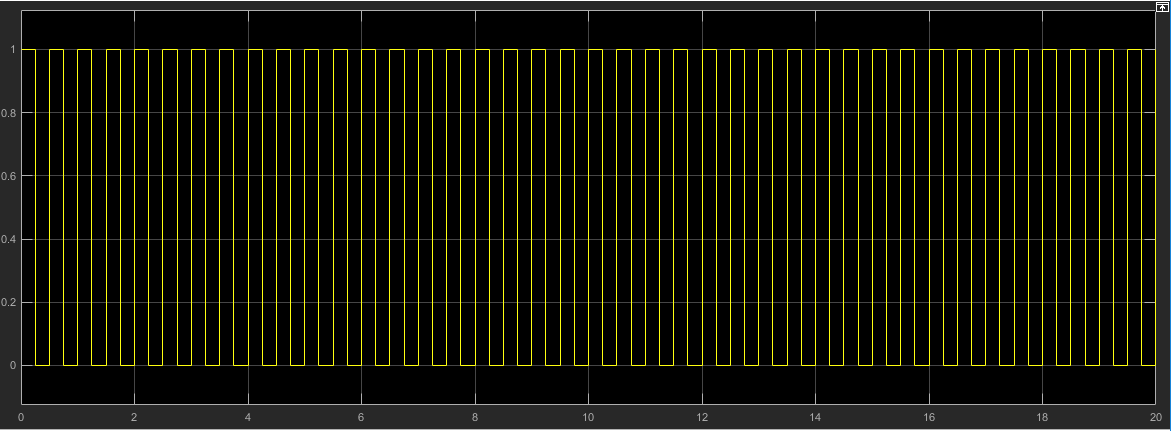
\includegraphics[width=0.5\linewidth]{screen/015.png}}
\caption{Схема для исследования прямоугольного дискретного сигнала.}
\label{015}
\end{figure}

В окне симуляции видим смоделированный прямоугольный сигнал.

\subsubsection{Получение спектра дискретного сигнала}

На рисунке \ref{013} изображена схема, предназначенная для получения спектра дискретного сигнала.

Результаты симуляции изображены на рисунке \ref{016}.

\begin{figure}[H]
\center{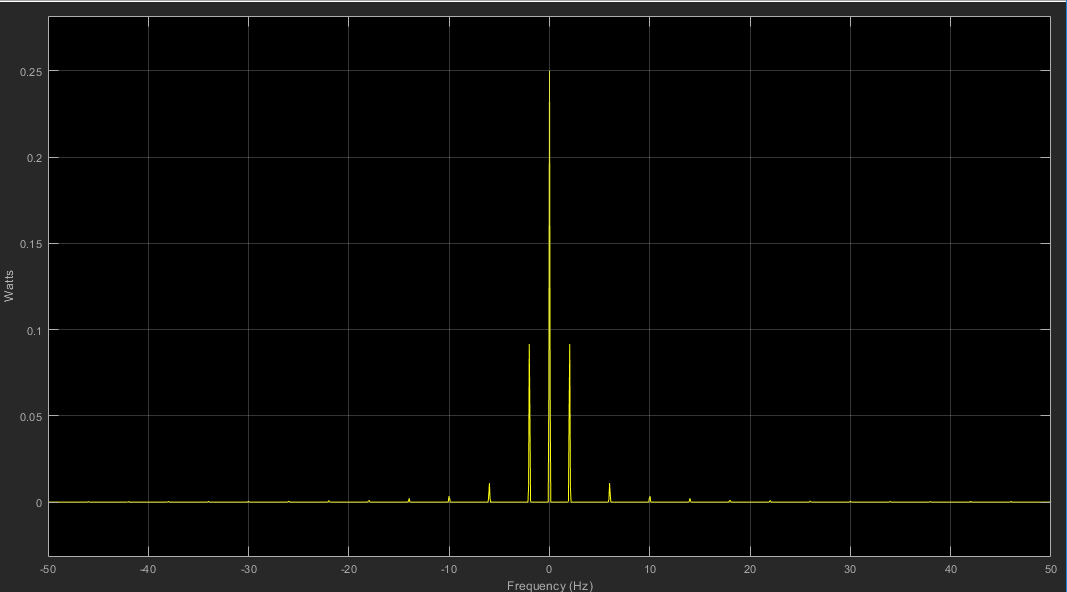
\includegraphics[width=0.5\linewidth]{screen/016.png}}
\caption{Схема для исследования прямоугольного дискретного сигнала.}
\label{016}
\end{figure}

Необходимо изменить параметры сигнала, чтобы узнать как будет изменяться спектр.

Изменим период сигнала с 50 на 30.

\begin{figure}[H]
\center{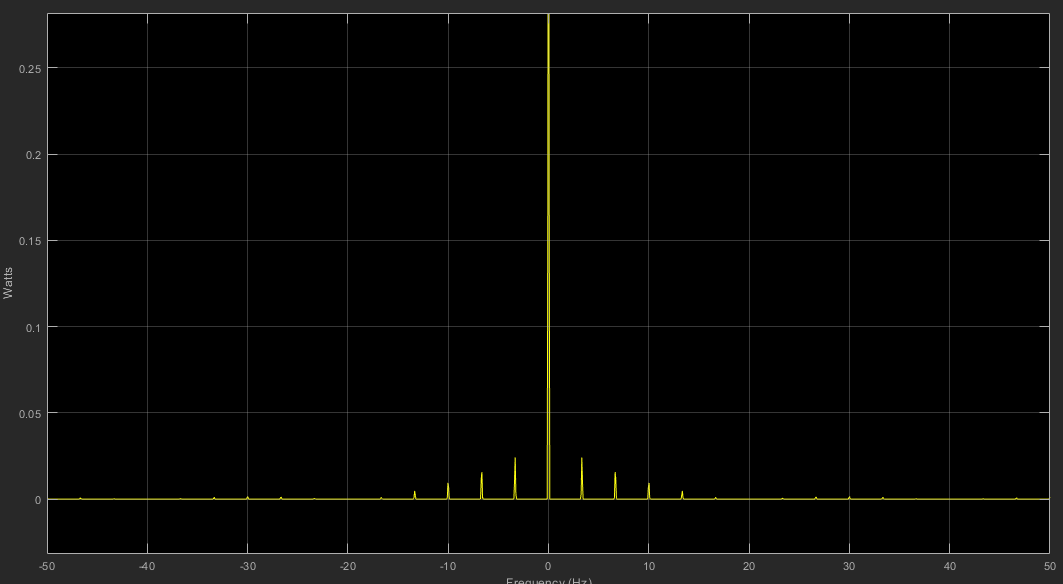
\includegraphics[width=0.5\linewidth]{screen/017.png}}
\caption{Схема для исследования прямоугольного дискретного сигнала.}
\label{017}
\end{figure}


Изменим длину импульса с 25 на 5.

\begin{figure}[H]
\center{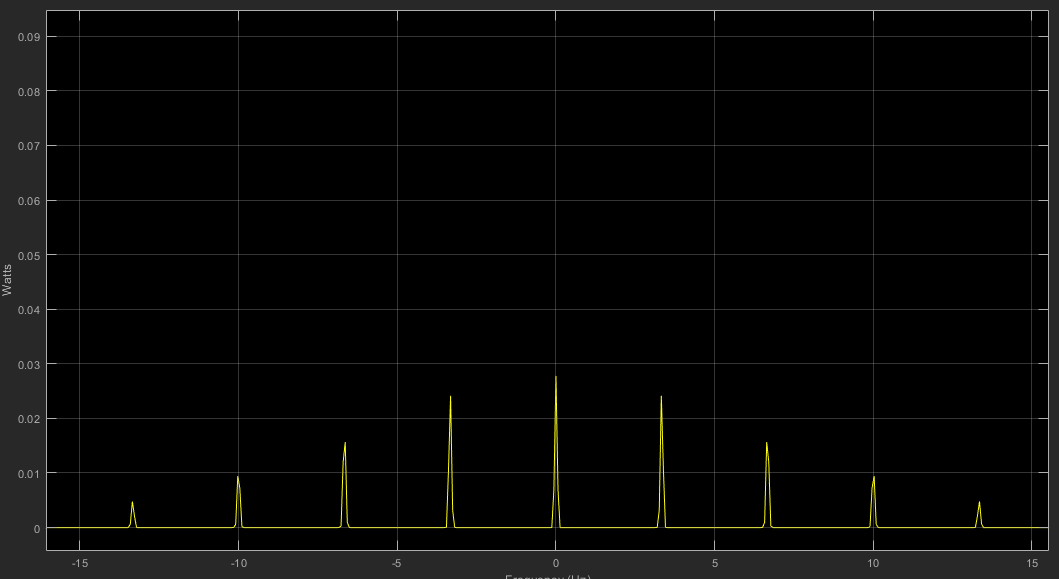
\includegraphics[width=0.5\linewidth]{screen/018.png}}
\caption{Схема для исследования прямоугольного дискретного сигнала.}
\label{018}
\end{figure}


Были получены спектры дискретных прямоугольных сигналов с различными параметрами.

\section{Корреляция}

\subsection{Сравнение алгоритмов прямой и быстрой корреляции}
В приведённом ниже коде сравниваются алгоритмы прямой и быстрой корреляции. Необходимо найти синхропосылку [101] в сигнале [0001010111000010].

\begin{figure}[H]
\center{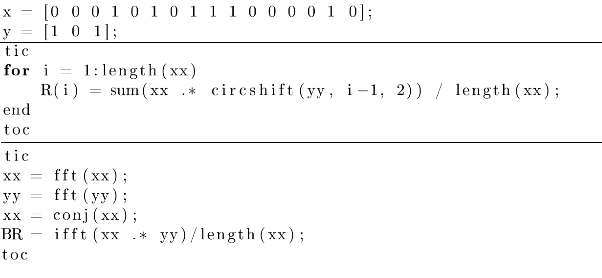
\includegraphics[width=0.5\linewidth]{screen/019.png}}
\caption{Код алгоритмов прямой и быстрой корреляции в MatLab.}
\label{019}
\end{figure}

Из результатов работы программы выяснили, что посылка в сигнале находится дважды. Это показали оба алгоритма.

Время выполнения прямой и быстрой корреляции 0.272ms и 0.103ms соответственно. 
Алгоритм быстрой корреляции нашёл посылки в сигнале значительно быстрее, чем в алгоритме прямой корреляции.

\section{Выводы}

Сигналы используются для передачи информации. Они бывают дискретные и непрерывные, периодические и непериодические, конечные и бесконечные. Дискретный сигнал имеет периодический спектр, периодический сигнал имеет дискретный спектр, а сигнал, который ограничен во времени имеет бесконечный спектр.
В ходе работы была проведено моделирование различных непрерывных и дискретных сигналов, для дискретных был получен спектр сигнала. Сигналы были смоделированы при помощи средств среды Simulink.

Корреляционный анализ дает возможность установить в сигналах наличие связи. Методы корреляции применяются при анализе случайных процессов для выявления неслучайных составляющих и оценки неслучайных параметров этих процессов.
Преобразования Фурье в телекоммуникационных технологиях применяются для обработки изображений и звука, для модуляции и демодуляции данных при фильтрации сигналов и передаче по различным каналам связи.

\end{document}
